\chapter{Diagramas binários sólido--líquido}\label{ch:b2:solid-liquid-diagrams}

O estanho funde a \qty{232}{\degreeCelsius} e o chumbo a \qty{327}{\degreeCelsius};
no entanto, a velha solda dos eletricistas, uma mistura dos dois, funde a
\qty{182}{\degreeCelsius}, abaixo de ambos. O sal espalhado em uma estrada
derrete o gelo, mas só até cerca de \qty{-21}{\degreeCelsius}; em uma noite mais
fria, ele não faz nada. O cobre e o níquel, por sua vez, se misturam em
qualquer proporção mesmo no estado sólido, e suas ligas fundem em uma faixa
de temperaturas entre as dos dois metais. Os diagramas deste capítulo dizem,
para cada par, quais sólidos cristalizam a partir de um líquido que esfria,
a que temperaturas e em que quantidades --- o conhecimento por trás de toda
peça fundida, de toda junta de solda e de toda liga de baixo ponto de fusão.

\begin{recall}
\Cref{ch:b2:chemical-potential}: \omterm{def:b2:chemical-potential:chemical-potential}{potencial químico} de um componente em uma
\omterm{def:b2:chemical-potential:ideal-mixture}{mistura ideal}, crioscopia. \Cref{ch:b2:equilibrium-shifts}: a \omterm{def:b2:equilibrium-shifts:variance}{variância}.
\Cref{ch:b2:liquid-vapour-diagrams}: \omterm{def:b2:liquid-vapour-diagrams:binary-diagram}{diagramas binários}, linhas de amarração e
\omterm{thm:b2:liquid-vapour-diagrams:lever}{regra da alavanca}. O volume do 1.º ano: ligação metálica, ligas
substitucionais e intersticiais, tipos de cristais.
\end{recall}

\begin{omfigure}
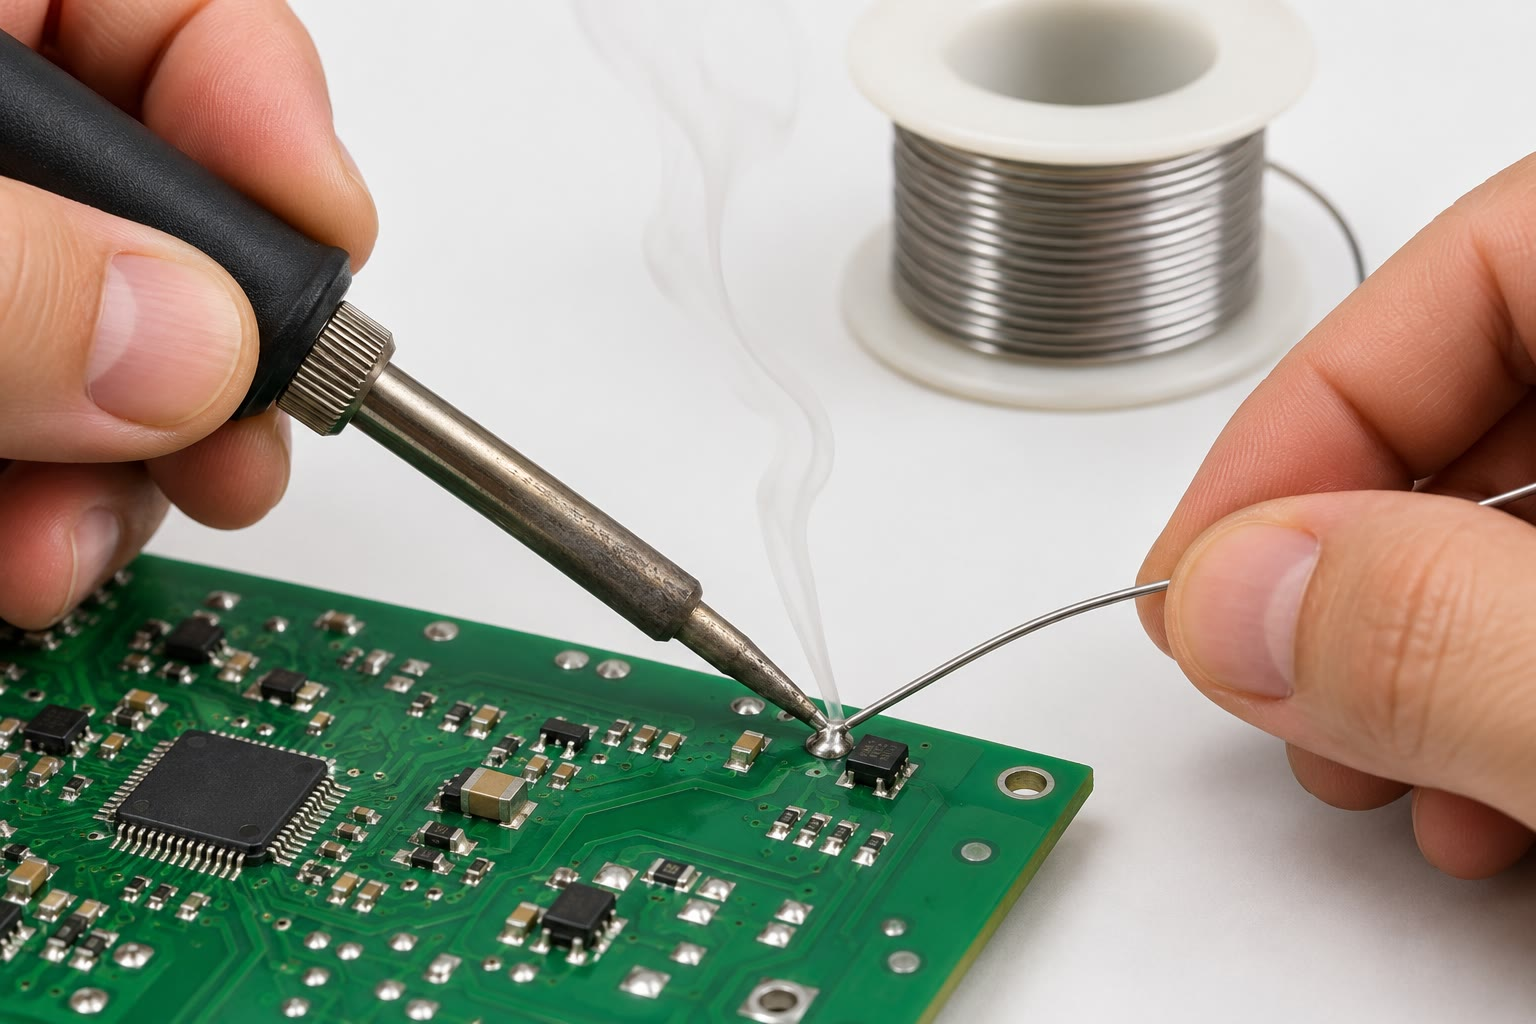
\includegraphics[width=0.6\linewidth]{images/book3/ai/b2-08-soldering.jpg}

{\small Soldagem de um componente em uma placa de circuito: o fio de solda
funde ao tocar o ferro quente e a junta solidifica em um segundo quando o
ferro é retirado --- porque a liga funde a uma única temperatura, baixa.}
\end{omfigure}

\section{Análise térmica}

\begin{definition}[Análise térmica]\label{def:b2:solid-liquid-diagrams:cooling-curve}
A \emph{análise térmica}\index{analise termica@análise térmica} determina as temperaturas
das mudanças de estado de uma amostra a partir de sua temperatura registrada
enquanto ela é aquecida ou resfriada a uma taxa constante. O registro da
temperatura em função do tempo durante um resfriamento lento é uma
\emph{curva de resfriamento}\index{curva de resfriamento}.
\end{definition}

Longe de qualquer mudança de estado, a amostra esfria de modo regular. Quando
um sólido começa a cristalizar, o calor de cristalização desacelera o
resfriamento: a curva mostra uma quebra de inclinação, ou para em uma
temperatura constante por algum tempo --- um \textit{patamar} --- se a
solidificação ocorre a temperatura fixa.

\begin{proposition}[Patamares]\label{prop:b2:solid-liquid-diagrams:plateaus}
A pressão fixa, uma substância pura solidifica a temperatura constante, assim
como um líquido binário do qual dois sólidos cristalizam juntos. Um líquido
binário do qual um único sólido cristaliza solidifica em uma faixa de
temperaturas.
\end{proposition}

\begin{proof}
Com a pressão fixa, a \omterm{def:b2:equilibrium-shifts:variance}{variância} é $v = n - r + 1 - \varphi$. Substância
pura, líquido + sólido: $v = 1 + 1 - 2 = 0$. Binário, líquido + dois sólidos:
$v = 2 + 1 - 3 = 0$. Binário, líquido + um sólido: $v = 2 + 1 - 2 = 1$: a
temperatura varia à medida que a composição do líquido varia. Uma \omterm{def:b2:equilibrium-shifts:variance}{variância} 0
significa que a temperatura não pode mudar enquanto todas as fases estão
presentes: o calor retirado é fornecido pela solidificação, até que uma fase
desapareça.
\end{proof}

\begin{omfigure}
\begin{tikzpicture}[font=\small, x=0.55cm, y=0.05cm]
  \foreach \dx/\name in {0/metal puro, 9/{mistura, um sólido antes}, 18/mistura eutética} {
    \draw[->] (\dx,0) -- (\dx+7.5,0) node[below left, font=\scriptsize] {$t$};
    \draw[->] (\dx,0) -- (\dx,62) node[above, font=\scriptsize] {$T$};
    \node[font=\scriptsize] at (\dx+3.8,-8) {\name};
  }
  % pure: cool, plateau at 40, cool
  \draw[omDef, thick] (0,58) .. controls (1,48) and (1.6,42) .. (2,40) -- (4.5,40) .. controls (5.2,32) and (6,24) .. (7,20);
  \node[font=\scriptsize, anchor=south] at (3.25,40.5) {patamar};
  % mixture: cool, break at 48, slow fall, plateau at 30, cool
  \draw[omDef, thick] (9,58) .. controls (9.6,53) and (9.9,50) .. (10.2,48)
     .. controls (11,42) and (11.6,35) .. (12.3,30) -- (14.2,30) .. controls (14.9,23) and (15.6,17) .. (16.5,14);
  \node[font=\scriptsize, anchor=west] at (10.4,49.5) {quebra};
  \node[font=\scriptsize, anchor=south] at (13.25,30.5) {eutético};
  % eutectic: plateau at 30
  \draw[omDef, thick] (18,58) .. controls (19,46) and (19.8,36) .. (20.5,30) -- (24,30) .. controls (24.7,23) and (25.4,17) .. (26.2,14);
  \node[font=\scriptsize, anchor=south] at (22.25,30.5) {patamar};
\end{tikzpicture}

{\small \omterm{def:b2:solid-liquid-diagrams:cooling-curve}{Curvas de resfriamento}, esquemáticas. Um metal puro solidifica em um
patamar. Uma mistura mostra uma quebra de inclinação quando aparece o
primeiro sólido, depois o resfriamento lento de um líquido que solidifica em
uma faixa de temperaturas, depois o patamar do eutético. Um líquido de
composição eutética solidifica em um único patamar, como uma substância pura.}
\end{omfigure}

\begin{method}[Construir um diagrama a partir de curvas de resfriamento]\label{met:b2:solid-liquid-diagrams:diagram-from-curves}
\begin{enumerate}
  \item Registre \omterm{def:b2:solid-liquid-diagrams:cooling-curve}{curvas de resfriamento} para uma série de composições,
        incluindo os componentes puros.
  \item Em um gráfico (composição, temperatura), marque para cada composição a
        temperatura da primeira quebra (o início da cristalização) e de
        cada patamar.
  \item Una os pontos de início de cristalização: é o \omterm{def:b2:solid-liquid-diagrams:liquidus}{liquidus}. Una os fins
        de solidificação: o \omterm{def:b2:solid-liquid-diagrams:liquidus}{solidus}. Um patamar encontrado na mesma
        temperatura para muitas composições é uma reta invariante (um eutético).
  \item O comprimento do patamar eutético, máximo na composição eutética,
        localiza essa composição.
\end{enumerate}
\end{method}

\section{Miscibilidade total no sólido}

\begin{definition}[Solução sólida]\label{def:b2:solid-liquid-diagrams:solid-solution}
Uma \emph{solução sólida}\index{solucao solida@solução sólida} é uma única fase cristalina de
composição variável, na qual átomos de um componente substituem átomos do
outro nos sítios da mesma rede (substitucional) ou ocupam os interstícios
dessa rede (intersticial).
\end{definition}

O cobre e o níquel têm a mesma estrutura cúbica de faces centradas e átomos de
raios próximos: formam uma \omterm{def:b2:solid-liquid-diagrams:solid-solution}{solução sólida} substitucional em qualquer composição.

\begin{definition}[Liquidus e solidus]\label{def:b2:solid-liquid-diagrams:liquidus}
Em um diagrama sólido--líquido, o \emph{liquidus}\index{liquidus} é a curva
acima da qual tudo é líquido; ele dá a composição do líquido em equilíbrio
com um sólido. O \emph{solidus}\index{solidus} é a curva abaixo da qual tudo
é sólido; onde o sólido é uma solução, ele dá a composição do sólido em
equilíbrio com o líquido.
\end{definition}

\begin{proposition}[O fuso]\label{prop:b2:solid-liquid-diagrams:lens}
Se os dois componentes formam soluções ideais no líquido e no sólido, o
\omterm{def:b2:solid-liquid-diagrams:liquidus}{liquidus} e o \omterm{def:b2:solid-liquid-diagrams:liquidus}{solidus} unem os dois pontos de fusão e delimitam um domínio
bifásico em forma de fuso; a cada temperatura, as frações molares $x_i$ de
cada componente no líquido e no sólido estão relacionadas por
\[
  \frac{x_i^{\ell}}{x_i^{s}} = \exp\left[-\frac{\Delta_{\text{fus}}H_i}{R}\left(\frac1T - \frac1{T_i^*}\right)\right] .
\]
\end{proposition}

\begin{proof}
O \omterm{def:b2:chemical-potential:chemical-potential}{potencial químico} de $i$ é o mesmo nas duas fases, $\mu_i^{*,s} +
RT\ln x_i^s = \mu_i^{*,\ell} + RT\ln x_i^\ell$, logo $RT\ln(x_i^\ell/x_i^s) =
-(\mu_i^{*,\ell} - \mu_i^{*,s}) = -\Delta_{\text{fus}}G_i(T)$ e, com
$\Delta_{\text{fus}}H_i$ constante, $\Delta_{\text{fus}}G_i = \Delta_{\text{fus}}H_i(1 - T/T_i^*)$.
Junto com $x_1 + x_2 = 1$ em cada fase, as duas relações fixam as duas
composições a cada $T$ (resolvidas numericamente para a figura); que as
curvas resultantes formam um fuso é admitido.
\end{proof}

\begin{omfigure}
\begin{tikzpicture}
\begin{axis}[omphase, width=0.62\linewidth, height=7cm, ymin=1050, ymax=1480,
  xlabel={$x$ (níquel)}, ylabel={$T$ (\unit{\degreeCelsius})}]
\addplot[omliquidus] table[x=xl, y=T] {figdata/out/bachelor-2-solid-liquid-a.dat};
\addplot[omsolidus] table[x=xs, y=T] {figdata/out/bachelor-2-solid-liquid-a.dat};
\draw[tieline] (axis cs:0.541,1300) -- (axis cs:0.609,1300);
\fill (axis cs:0.58,1300) circle (1.3pt);
\node[font=\scriptsize] at (axis cs:0.25,1400) {líquido};
\node[font=\scriptsize] at (axis cs:0.8,1150) {solução sólida};
\node[font=\scriptsize, anchor=east] at (axis cs:0.5,1330) {liquidus};
\node[font=\scriptsize, anchor=west] at (axis cs:0.66,1290) {solidus};
\node[font=\scriptsize, anchor=west] at (axis cs:0.03,1080) {\qty{1085}{\degreeCelsius}};
\draw[black!50] (axis cs:0.005,1084) -- (axis cs:0.03,1080);
\node[font=\scriptsize, anchor=south east] at (axis cs:1.0,1456) {\qty{1455}{\degreeCelsius}};
\end{axis}
\end{tikzpicture}

{\small Cobre--níquel, calculado para soluções sólida e líquida ideais a partir
dos pontos de fusão e das entalpias de fusão dos dois metais. A
\qty{1300}{\degreeCelsius}, uma liga de composição 0.58 se divide em um líquido
de 0.541 e um sólido de 0.609 (linha de amarração tracejada).}
% ledger: tfus:Cu, dfus:Cu, tfus:Ni, dfus:Ni
\end{omfigure}

\begin{method}[Ler um diagrama sólido--líquido]\label{met:b2:solid-liquid-diagrams:read-solid-liquid}
\begin{enumerate}
  \item Siga para baixo, a partir do líquido, a vertical da composição global.
  \item No \omterm{def:b2:solid-liquid-diagrams:liquidus}{liquidus}, aparece o primeiro sólido; sua composição é lida na outra
        extremidade da linha de amarração (o \omterm{def:b2:solid-liquid-diagrams:liquidus}{solidus}, ou um componente puro).
  \item No domínio bifásico, leia as duas composições nas extremidades da
        linha de amarração e as proporções pela \omterm{thm:b2:liquid-vapour-diagrams:lever}{regra da alavanca}, em mols
        com frações molares, em massa com frações mássicas.
  \item Em uma reta invariante horizontal, a temperatura para até que uma
        fase tenha desaparecido; abaixo dela, leia o novo par de fases.
\end{enumerate}
\end{method}

\begin{example}[Uma liga a \qty{1300}{\degreeCelsius}]\label{ex:b2:solid-liquid-diagrams:lever}
Para a liga de fração molar de níquel 0.58 a \qty{1300}{\degreeCelsius}, a
fração dos átomos no sólido é $(0.58 - 0.541)/(0.609 - 0.541) = 0.57$.
O primeiro sólido a aparecer, perto de \qty{1315}{\degreeCelsius}, é mais rico
em níquel que a liga, e o último líquido, mais pobre.
\end{example}

O diagrama descreve o equilíbrio, que em um sólido é lento: os primeiros
cristais, ricos em níquel, são recobertos por camadas cada vez mais pobres
nele à medida que o líquido muda, e a difusão no sólido não tem tempo de
uniformizá-las. Uma peça fundida resfriada rapidamente é formada por cristais
\textit{zonados}, com gradiente do centro para a borda; um longo aquecimento
abaixo do \omterm{def:b2:solid-liquid-diagrams:liquidus}{solidus} os homogeneíza.

\section{Nenhuma miscibilidade no sólido: o eutético}

Quando os dois sólidos não se misturam de modo algum, cada componente
cristaliza puro, e o \omterm{def:b2:solid-liquid-diagrams:liquidus}{liquidus} tem dois ramos, um para cada sólido.

\begin{theorem}[Schröder--van Laar]\label{thm:b2:solid-liquid-diagrams:schroder}
Se um componente A cristaliza puro a partir de uma mistura líquida ideal, o
\omterm{def:b2:solid-liquid-diagrams:liquidus}{liquidus} no qual aparece o sólido A é dado por
\[
  \ln x_A = -\frac{\Delta_{\text{fus}}H_A}{R}\Big(\frac1T - \frac1{T_A^*}\Big),
\]
sendo $x_A$ a fração molar de A no líquido, $T_A^*$ e
$\Delta_{\text{fus}}H_A$ o ponto de fusão e a entalpia de fusão de A puro
(tomada como constante).
\end{theorem}

\begin{proof}
No equilíbrio, o \omterm{def:b2:chemical-potential:chemical-potential}{potencial químico} de A sólido puro é igual ao de A no
líquido: $\mu_A^{*,s}(T) = \mu_A^{*,\ell}(T) + RT\ln x_A$. Logo $R\ln x_A =
-\Delta_{\text{fus}}G_A(T)/T$. Pela relação de Gibbs--Helmholtz, $d(\Delta_{\text{fus}}G_A/T)/
dT = -\Delta_{\text{fus}}H_A/T^2$; integrando de $T_A^*$, onde
$\Delta_{\text{fus}}G_A = 0$, até $T$, obtém-se $\Delta_{\text{fus}}G_A/T =
\Delta_{\text{fus}}H_A(1/T - 1/T_A^*)$.
\end{proof}

Para uma solução diluída, $\ln x_A = \ln(1 - x_B) \approx -x_B$ e $1/T -
1/T_A^* \approx -\Delta T/T_A^{*2}$: $\Delta T = RT_A^{*2}x_B/\Delta_{\text{fus}}H_A$,
a lei crioscópica do \cref{ch:b2:chemical-potential}. Para o benzeno ($T^* =
\qty{278.64}{K}$, $\Delta_{\text{fus}}H = \qty{9.87}{kJ/mol}$, $M =
\qty{78.11}{g/mol}$), a \omterm{def:b2:chemical-potential:colligative}{constante crioscópica} $RT^{*2}M/\Delta_{\text{fus}}H$
resulta em \qty{5.11}{K.kg/mol}.
% ledger: tfus:benzene, dfus:benzene

\begin{definition}[Eutético]\label{def:b2:solid-liquid-diagrams:eutectic}
O \emph{ponto eutético}\index{ponto eutetico@ponto eutético} de um sistema binário é o
ponto em que o líquido está em equilíbrio com dois sólidos ao mesmo tempo; é
a temperatura mais baixa na qual um líquido existe nessa parte do diagrama.
Um líquido de composição eutética, e a mistura fina e íntima dos dois
sólidos na qual ele solidifica, chamam-se \emph{mistura
eutética}\index{mistura eutetica@mistura eutética}.
\end{definition}

\begin{corollary}[O eutético é onde os ramos do liquidus se encontram]\label{cor:b2:solid-liquid-diagrams:eutectic}
Para dois componentes imiscíveis no sólido e ideais no líquido, a
temperatura eutética $T_E$ e a composição eutética são a solução de
$x_A(T_E) + x_B(T_E) = 1$, sendo cada $x$ dado pela equação de
Schröder--van Laar de seu próprio sólido.
\end{corollary}

\begin{proof}
No eutético, o líquido está saturado dos dois sólidos: ele está nos dois
ramos ao mesmo tempo, com a mesma composição lida em A e em B.
\end{proof}

\begin{omfigure}
\begin{tikzpicture}
\begin{axis}[omphase, width=0.62\linewidth, height=6.5cm, ymin=-25, ymax=85,
  xlabel={$x$ (naftaleno)}, ylabel={$T$ (\unit{\degreeCelsius})}]
\addplot[omliquidus] table[x=x, y=T] {figdata/out/bachelor-2-solid-liquid-b-benzene.dat};
\addplot[omliquidus] table[x=x, y=T] {figdata/out/bachelor-2-solid-liquid-b-naphthalene.dat};
\draw[thick] (axis cs:0,-3.55) -- (axis cs:1,-3.55);
\fill (axis cs:0.133,-3.55) circle (1.5pt);
\node[font=\scriptsize, anchor=north] at (axis cs:0.133,-4.5) {E};
\node[font=\scriptsize] at (axis cs:0.45,72) {líquido};
\node[font=\scriptsize, align=center] at (axis cs:0.65,22) {líquido + naftaleno\\ sólido};
\node[font=\scriptsize, anchor=south west] at (axis cs:0.08,45) {líquido + benzeno sólido};
\draw[thin] (axis cs:0.12,45) -- (axis cs:0.06,0.8);
\node[font=\scriptsize] at (axis cs:0.55,-15) {benzeno sólido + naftaleno sólido};
\end{axis}
\end{tikzpicture}

{\small Benzeno--naftaleno, calculado com a equação de Schröder--van Laar
para cada sólido. Os dois ramos se encontram no eutético E,
\qty{-3.5}{\degreeCelsius} e 0.13 de naftaleno, abaixo do qual tudo é sólido.}
% ledger: tfus:benzene, dfus:benzene, tfus:naphthalene, dfus:naphthalene
\end{omfigure}

\begin{example}[Resfriamento de uma mistura benzeno--naftaleno]\label{ex:b2:solid-liquid-diagrams:naphthalene}
Um líquido de fração molar de naftaleno 0.5 esfria até o ramo do naftaleno
no \omterm{def:b2:solid-liquid-diagrams:liquidus}{liquidus}, perto de \qty{46}{\degreeCelsius}, onde o naftaleno sólido puro
começa a cristalizar. O líquido, perdendo naftaleno, desce ao longo do ramo;
a \qty{-3.5}{\degreeCelsius} ele atinge o eutético, e o restante solidifica a
temperatura constante na \omterm{def:b2:solid-liquid-diagrams:eutectic}{mistura eutética}. Pela \omterm{thm:b2:liquid-vapour-diagrams:lever}{regra da alavanca}, logo
acima do eutético, o naftaleno sólido representa $(0.5 - 0.133)/(1 - 0.133) =
42~\%$ dos mols, e o líquido eutético, 58~\%.
\end{example}

\begin{proposition}[Duração do patamar eutético]\label{prop:b2:solid-liquid-diagrams:plateau-length}
Para amostras de mesma massa resfriadas com a mesma taxa de retirada de calor,
a duração do patamar eutético é proporcional à quantidade de líquido que
atinge o eutético, máxima para a composição eutética e nula para os
componentes puros.
\end{proposition}

\begin{proof}
No patamar, a temperatura é constante: o calor retirado, $\Phi\,\Delta t$
a uma taxa constante $\Phi$, é o calor liberado pela solidificação do
líquido eutético, $m_E\,\Delta_{\text{fus}}h_E$. Logo $\Delta t = m_E\,\Delta_{\text{fus}}h_E/
\Phi$, proporcional à massa $m_E$ de líquido eutético, dada pela \omterm{thm:b2:liquid-vapour-diagrams:lever}{regra
da alavanca}.
\end{proof}

\section{Miscibilidade parcial e compostos definidos}

A maioria dos pares de metais não é nem totalmente miscível nem totalmente
imiscível no sólido: cada um dissolve um pouco do outro. O chumbo dissolve
até 19~\% de estanho em massa, o estanho até 3.4~\% de chumbo. O diagrama
contém então duas \omterm{def:b2:solid-liquid-diagrams:solid-solution}{soluções sólidas}, (Pb) e (Sn), e um eutético entre elas; a
reta eutética deixa de alcançar os lados do diagrama e para nos limites das
\omterm{def:b2:solid-liquid-diagrams:solid-solution}{soluções sólidas}.

\begin{omfigure}
\begin{tikzpicture}[font=\small, x=0.075cm, y=0.022cm]
  \draw[->] (0,0) -- (106,0) node[right] {\% Sn (massa)};
  \draw[->] (0,0) -- (0,360) node[above] {$T$ (\unit{\degreeCelsius})};
  \foreach \t in {100,200,300} \draw (0,\t) -- (-1.5,\t) node[left, font=\scriptsize] {\t};
  \foreach \w in {0,20,40,60,80,100} \draw (\w,0) -- (\w,-5) node[below, font=\scriptsize] {\w};
  % invariant points (NIST): Pb 327.5, Sn 231.9, eutectic 182.2 at 62.13; limits 18.91 and 96.59
  \draw[omliquidus] (0,327.5) .. controls (25,290) and (45,235) .. (62.13,182.2);
  \draw[omliquidus] (100,231.9) .. controls (85,215) and (72,200) .. (62.13,182.2);
  \draw[omsolidus] (0,327.5) .. controls (8,280) and (14,220) .. (18.91,182.2);
  \draw[omsolidus] (100,231.9) .. controls (98.5,215) and (97.5,200) .. (96.59,182.2);
  \draw[thick] (18.91,182.2) -- (96.59,182.2);
  \draw[omsolidus, densely dashed] (18.91,182.2) .. controls (12,120) and (6,60) .. (3,20);
  \draw[omsolidus, densely dashed] (96.59,182.2) .. controls (98.5,120) and (99.3,60) .. (99.6,20);
  \fill (62.13,182.2) circle (1.5pt);
  \fill (18.91,182.2) circle (1.2pt); \fill (96.59,182.2) circle (1.2pt);
  \node[anchor=south, font=\scriptsize] at (62.13,186) {E};
  \node[font=\scriptsize] at (55,300) {líquido};
  \node[font=\scriptsize] at (6,150) {(Pb)};
  \node[font=\scriptsize] at (103,140) {(Sn)};
  \node[font=\scriptsize] at (28,235) {L + (Pb)};
  \node[font=\scriptsize] at (84,192) {L + (Sn)};
  \node[font=\scriptsize] at (55,100) {(Pb) + (Sn)};
  % cooling path at 40 %
  \draw[->, omProp, thick] (40,340) -- (40,30);
  \node[font=\scriptsize, omProp, anchor=south] at (40,342) {40~\%};
  \node[font=\scriptsize, anchor=north east] at (16.6,179) {18.9};
  \node[font=\scriptsize, anchor=north] at (62.13,178) {62.1};
  \node[font=\scriptsize, anchor=north east] at (95.8,178) {96.6};
  \node[font=\scriptsize, anchor=west] at (101,182.2) {\qty{182.2}{\degreeCelsius}};
\end{tikzpicture}

{\small O diagrama chumbo--estanho, traçado por seus pontos invariantes: pontos
de fusão do chumbo (\qty{327.5}{\degreeCelsius}) e do estanho (\qty{231.9}{\degreeCelsius}),
eutético E a \qty{182.2}{\degreeCelsius} e 62.1~\% de estanho, limites das
\omterm{def:b2:solid-liquid-diagrams:solid-solution}{soluções sólidas} na temperatura eutética (18.9~\% e 96.6~\% de estanho). As
curvas entre esses pontos, e os limites de solubilidade tracejados abaixo do
eutético, são traçados esquematicamente. Seta: o resfriamento de uma solda
com 40~\%.}
% ledger: eut:Pb-Sn.T, eut:Pb-Sn.wL, eut:Pb-Sn.wPb, eut:Pb-Sn.wSn, tfus:Pb, tfus:Sn
\end{omfigure}

Uma solda com 40~\% de estanho começa a solidificar no \omterm{def:b2:solid-liquid-diagrams:liquidus}{liquidus} depositando
cristais da solução rica em chumbo (Pb); o líquido se enriquece em estanho
até que, a \qty{182.2}{\degreeCelsius}, atinge a composição eutética e
solidifica em uma mistura fina de lamelas de (Pb) e (Sn), em torno dos
cristais primários.

\begin{omfigure}
\begin{tikzpicture}[font=\small]
  \begin{scope}
    \clip (0,0) circle (2.2);
    \fill[gray!20] (-2.3,-2.3) rectangle (2.3,2.3);
    \foreach \k in {-24,...,24} \draw[gray!65, line width=1.1pt] (-2.4+0.2*\k,-2.4) -- ++(55:6);
    \foreach \cx/\cy/\r/\a in {-0.9/0.8/0.55/10, 0.7/1.0/0.45/40, 0.2/-0.6/0.6/-20, -1.1/-0.9/0.4/70, 1.3/-0.3/0.35/5} {
      \fill[omDef!35, draw=omDef, rotate around={\a:(\cx,\cy)}] (\cx,\cy) ellipse ({\r} and {0.7*\r});
    }
  \end{scope}
  \draw[thick] (0,0) circle (2.2);
  \draw[<-, omProp, thick] (0.7,1.0) -- (3.0,1.6) node[right, text=black] {cristal primário de (Pb)};
  \draw[<-, omProp, thick] (1.6,0.9) -- (3.0,0.5) node[right, text=black, align=left] {eutético: lamelas\\ alternadas de (Pb) e (Sn)};
\end{tikzpicture}

{\small A microestrutura de uma solda com 40~\% de estanho após resfriamento
lento, esquemática: cristais primários de (Pb), formados entre o \omterm{def:b2:solid-liquid-diagrams:liquidus}{liquidus} e o
eutético, em uma matriz de eutético feita de finas placas alternadas das
duas \omterm{def:b2:solid-liquid-diagrams:solid-solution}{soluções sólidas}.}
\end{omfigure}

\begin{definition}[Composto definido]\label{def:b2:solid-liquid-diagrams:defined-compound}
Um \emph{composto definido}\index{composto definido} é um sólido de composição
fixa $\mathrm{A}_a\mathrm{B}_b$ formado pelos dois componentes. Ele apresenta
\emph{fusão congruente}\index{fusao congruente@fusão congruente} quando funde em um
líquido de mesma composição: o \omterm{def:b2:solid-liquid-diagrams:liquidus}{liquidus} tem então um máximo nessa composição.
\end{definition}

Um composto de \omterm{def:b2:solid-liquid-diagrams:defined-compound}{fusão congruente} divide o diagrama em dois: cada metade, A com
$\mathrm{A}_a\mathrm{B}_b$ e $\mathrm{A}_a\mathrm{B}_b$ com B, é um diagrama
próprio, com seu próprio eutético. A composição do máximo, lida em fração
molar, dá a fórmula do composto.

\begin{omfigure}
\begin{tikzpicture}[font=\small, x=6cm, y=0.05cm]
  \draw[->] (0,0) -- (1.06,0) node[right] {$x_{\mathrm B}$};
  \draw[->] (0,0) -- (0,95) node[above] {$T$};
  \node[below, font=\scriptsize] at (0,0) {A}; \node[below, font=\scriptsize] at (1,0) {B};
  \node[below, font=\scriptsize] at (0.667,0) {$\tfrac23$};
  \draw[omliquidus] (0,70) .. controls (0.12,58) and (0.25,45) .. (0.35,35);
  \draw[omliquidus] (0.35,35) .. controls (0.45,62) and (0.58,79) .. (0.667,80);
  \draw[omliquidus] (0.667,80) .. controls (0.75,79) and (0.8,68) .. (0.85,50);
  \draw[omliquidus] (0.85,50) .. controls (0.9,56) and (0.95,62) .. (1,65);
  \draw[thick] (0,35) -- (0.667,35); \draw[thick] (0.667,50) -- (1,50);
  \draw[thick] (0.667,0) -- (0.667,80);
  \fill (0.35,35) circle[radius=1.5pt]; \fill (0.85,50) circle[radius=1.5pt];
  \fill (0.667,80) circle[radius=1.5pt];
  \node[anchor=north, font=\scriptsize] at (0.35,34) {E$_1$};
  \node[anchor=north, font=\scriptsize] at (0.85,49) {E$_2$};
  \node[anchor=south, font=\scriptsize] at (0.667,81) {$\mathrm{AB_2}$ funde};
  \node[font=\scriptsize] at (0.35,80) {líquido};
  \node[font=\scriptsize, align=center] at (0.33,15) {A +\\ $\mathrm{AB_2}$};
  \node[font=\scriptsize, align=center] at (0.84,25) {$\mathrm{AB_2}$\\ + B};
\end{tikzpicture}

{\small Diagrama esquemático com um \omterm{def:b2:solid-liquid-diagrams:defined-compound}{composto definido} $\mathrm{AB_2}$ (reta
vertical em $x_{\mathrm B} = 2/3$) com \omterm{def:b2:solid-liquid-diagrams:defined-compound}{fusão congruente} no máximo do
\omterm{def:b2:solid-liquid-diagrams:liquidus}{liquidus}. O diagrama é formado por dois diagramas eutéticos simples lado a
lado, com os eutéticos E$_1$ e E$_2$.}
\end{omfigure}

\section{Aplicações}

\paragraph{Soldas e ligas de baixo ponto de fusão.} Uma solda deve fundir
abaixo das peças que une e solidificar depressa, sem faixa pastosa: a
composição eutética é a escolha natural. O eutético estanho--chumbo funde a
\qty{182.2}{\degreeCelsius}; como o chumbo é tóxico, a eletrônica usa hoje
soldas sem chumbo, entre elas o eutético bismuto--estanho, que funde a
\qty{138.8}{\degreeCelsius} e contém 57~\% de bismuto em massa.
% ledger: eut:Pb-Sn.T, eut:Bi-Sn.T, eut:Bi-Sn.wL

\paragraph{Degelo.} O gelo e o sal formam um eutético: o eutético
gelo--di-hidrato de sal fica a \qty{252}{K} (\qty{-21}{\degreeCelsius}) e
23.3~\% de cloreto de sódio em massa. Acima dessa temperatura, o sal em
contato com o gelo forma uma salmoura cujo ponto de congelamento está abaixo
da temperatura da estrada, e o gelo derrete; abaixo dela, nenhum líquido pode
existir, e o sal é inútil.
% ledger: eut:NaCl-water.T, eut:NaCl-water.w

\paragraph{Cristalização.} O diagrama de um sal e da água se lê como
qualquer outro: resfriar uma solução saturada quente atravessa a curva de
solubilidade (o \omterm{def:b2:solid-liquid-diagrams:liquidus}{liquidus} do sal), e cristais puros do sal se depositam
enquanto as impurezas, diluídas demais para atingir seu próprio \omterm{def:b2:solid-liquid-diagrams:liquidus}{liquidus},
ficam na água-mãe. É a purificação por recristalização do volume do 1.º
ano, vista em um diagrama.

\begin{omfigure}
\begin{tikzpicture}
\begin{axis}[omphase, width=0.62\linewidth, height=6cm, xmin=0, xmax=100,
  ymin=90, ymax=285, xlabel={\% Bi (massa)}, ylabel={$T$ (\unit{\degreeCelsius})}]
\addplot[omliquidus] table[x=w, y=T] {figdata/out/bachelor-2-solid-liquid-d-Sn.dat};
\addplot[omliquidus] table[x=w, y=T] {figdata/out/bachelor-2-solid-liquid-d-Bi.dat};
\draw[densely dashed] (axis cs:0,119.5) -- (axis cs:100,119.5);
\fill[omThm] (axis cs:56.97,138.8) circle (2pt);
\node[font=\scriptsize, omThm, anchor=west] at (axis cs:64,129) {eutético avaliado};
\draw[omThm, thin] (axis cs:64,129) -- (axis cs:57.8,137.6);
\node[font=\scriptsize, anchor=north] at (axis cs:52,118) {modelo ideal};
\node[font=\scriptsize] at (axis cs:50,250) {líquido};
\end{axis}
\end{tikzpicture}

{\small Bismuto--estanho: o \omterm{def:b2:solid-liquid-diagrams:liquidus}{liquidus} previsto para sólidos puros e um líquido
ideal (Schröder--van Laar, em azul) leva a um eutético perto de
\qty{120}{\degreeCelsius}; o eutético avaliado (ponto vermelho) fica a
\qty{138.8}{\degreeCelsius} e 57~\% de bismuto.}
% ledger: tfus:Sn, dfus:Sn, tfus:Bi, dfus:Bi, eut:Bi-Sn.T, eut:Bi-Sn.wL
\end{omfigure}

\section{Exercícios}

\begin{exercise}[$\star$]\label{exo:b2:solid-liquid-diagrams:1}
No diagrama cobre--níquel, dê as fases presentes a
\qty{1300}{\degreeCelsius} para frações molares de níquel 0.40, 0.58 e 0.70.
\end{exercise}

\begin{exercise}[$\star$]\label{exo:b2:solid-liquid-diagrams:2}
\qty{2.00}{mol} de uma liga cobre--níquel de fração molar de níquel 0.58 são
mantidos a \qty{1300}{\degreeCelsius}. Calcule as quantidades de sólido e de
líquido e a quantidade de níquel em cada um.
\end{exercise}

\begin{exercise}[$\star$]\label{exo:b2:solid-liquid-diagrams:3}
Calcule a \omterm{def:b2:equilibrium-shifts:variance}{variância} a pressão fixa (a) de um metal puro enquanto ele
solidifica; (b) de uma liga cobre--níquel enquanto ela solidifica; (c) de um
líquido chumbo--estanho na reta eutética.
\end{exercise}

\begin{exercise}[$\star$]\label{exo:b2:solid-liquid-diagrams:4}
Esboce a \omterm{def:b2:solid-liquid-diagrams:cooling-curve}{curva de resfriamento} do estanho puro de \qty{300}{\degreeCelsius} a
\qty{100}{\degreeCelsius} e explique por que a temperatura para a
\qty{232}{\degreeCelsius}.
\end{exercise}

\begin{exercise}[$\star\star$]\label{exo:b2:solid-liquid-diagrams:5}
Com os dados do capítulo (benzeno \qty{278.64}{K}, \qty{9.87}{kJ/mol};
naftaleno \qty{353.2}{K}, \qty{19.1}{kJ/mol}), verifique que a
\qty{269.6}{K} as duas frações molares de Schröder--van Laar somam 1, e dê
a composição eutética.
\end{exercise}

\begin{exercise}[$\star\star$]\label{exo:b2:solid-liquid-diagrams:6}
Descreva o resfriamento de uma liga chumbo--estanho com 30~\% de estanho em
massa, do líquido até a temperatura ambiente, e calcule a fração mássica de
eutético que ela contém.
\end{exercise}

\begin{exercise}[$\star\star$]\label{exo:b2:solid-liquid-diagrams:7}
Que massa de cloreto de sódio por quilograma de água contém a salmoura
eutética? Por que salgar uma estrada é inútil a \qty{-25}{\degreeCelsius}?
\end{exercise}

\begin{exercise}[$\star\star$]\label{exo:b2:solid-liquid-diagrams:8}
No diagrama esquemático com o composto $\mathrm{AB_2}$, descreva o
resfriamento de líquidos com $x_{\mathrm B} = 0.5$ e $x_{\mathrm B} = 0.9$:
primeiro sólido, eutético atingido, sólidos no final.
\end{exercise}

\begin{exercise}[$\star\star$]\label{exo:b2:solid-liquid-diagrams:9}
No refino por zona, uma zona fundida é deslocada lentamente ao longo de uma
barra. Perto do níquel puro, a razão entre as frações molares de cobre no
sólido e no líquido em equilíbrio é de cerca de 0.78. Explique por que o
cobre é arrastado com a zona fundida e por que são necessárias várias
passagens.
\end{exercise}

\begin{exercise}[$\star\star\star$]\label{exo:b2:solid-liquid-diagrams:10}
Deduza a equação de Schröder--van Laar e depois mostre que, para um líquido
diluído, ela se reduz a $\Delta T = K_f\,b$, com $K_f = RT^{*2}M_A/\Delta_{\text{fus}}H_A$
e $b$ a molalidade do soluto; calcule $K_f$ para o benzeno.
\end{exercise}

\begin{exercise}[$\star\star\star$]\label{exo:b2:solid-liquid-diagrams:11}
O diagrama magnésio--chumbo tem um máximo do \omterm{def:b2:solid-liquid-diagrams:liquidus}{liquidus} em 19.0~\% de magnésio
em massa. Encontre a fórmula do composto.
\end{exercise}

\begin{exercise}[$\star\star\star$]\label{exo:b2:solid-liquid-diagrams:12}
Massas iguais de ligas chumbo--estanho são resfriadas nas mesmas condições.
A liga eutética apresenta um patamar de \qty{300}{s}; uma liga desconhecida,
um de \qty{120}{s}. Encontre as duas composições possíveis da liga
desconhecida e diga como distingui-las.
\end{exercise}

\section{Problema: A solda}

\begin{problem}[{Problema de fim de semana --- o diagrama chumbo--estanho a partir de
seus pontos invariantes, a solidificação de uma solda com 40~\% pela regra da
alavanca, uma solda sem chumbo bismuto--estanho prevista pelo modelo de
líquido ideal, e a escolha de uma solda}]
\label{pb:b2:solid-liquid-diagrams:1}
Dados (NIST, equilíbrios invariantes calculados): eutético chumbo--estanho a
\qty{182.2}{\degreeCelsius}, líquido com 62.13~\% de estanho em massa, em
equilíbrio com (Pb) com 18.91~\% e (Sn) com 96.59~\% de estanho; eutético
bismuto--estanho a \qty{138.8}{\degreeCelsius}, líquido com 56.97~\% de
bismuto. Pontos de fusão e entalpias de fusão: chumbo \qty{600.6}{K},
\qty{4.77}{kJ/mol}; estanho \qty{505.1}{K}, \qty{7.03}{kJ/mol}; bismuto
\qty{544.6}{K}, \qty{11.30}{kJ/mol}. Massas molares (\unit{g/mol}): Pb 207.2,
Sn 118.71, Bi 208.98.
% ledger: eut:Pb-Sn.T, eut:Pb-Sn.wL, eut:Pb-Sn.wPb, eut:Pb-Sn.wSn, eut:Bi-Sn.T, eut:Bi-Sn.wL, tfus:Pb, dfus:Pb, tfus:Sn, dfus:Sn, tfus:Bi, dfus:Bi, aw:Pb, aw:Sn, aw:Bi

\medskip
\noindent\textbf{Parte I --- O diagrama chumbo--estanho.}
\begin{enumerate}
  \item Converta os pontos de fusão do chumbo e do estanho para graus Celsius.
  \item Converta a composição eutética em fração molar de estanho.
  \item Marque em um gráfico (\% Sn em massa, $T$) os pontos de fusão, o
        eutético e as duas extremidades da reta eutética.
  \item Trace o diagrama e nomeie seus seis domínios.
  \item Escreva a transformação eutética no resfriamento.
  \item Calcule a \omterm{def:b2:equilibrium-shifts:variance}{variância} na reta eutética a pressão fixa.
\end{enumerate}

\medskip
\noindent\textbf{Parte II --- Resfriamento de uma solda com 40~\%.}
\begin{enumerate}[resume]
  \item Que sólido aparece primeiro, e por que não é chumbo puro?
  \item Como varia a composição do líquido durante o resfriamento até o
        eutético?
  \item Logo acima de \qty{182.2}{\degreeCelsius}: quais fases, de que
        composições?
  \item Calcule suas frações mássicas.
  \item Logo abaixo: quais fases, de que composições e em que frações
        mássicas?
  \item Que fração da liga é formada pelo constituinte eutético, e que fração
        por cristais primários de (Pb)?
  \item Esboce a \omterm{def:b2:solid-liquid-diagrams:cooling-curve}{curva de resfriamento} e compare seu patamar com o da liga
        eutética.
\end{enumerate}

\medskip
\noindent\textbf{Parte III --- Uma solda sem chumbo pelo modelo de líquido ideal.}
\begin{enumerate}[resume]
  \item Escreva a equação de Schröder--van Laar para o \omterm{def:b2:solid-liquid-diagrams:liquidus}{liquidus} do estanho.
  \item Escreva-a para o \omterm{def:b2:solid-liquid-diagrams:liquidus}{liquidus} do bismuto.
  \item Escreva a condição que define o eutético.
  \item Calcule a soma das duas frações molares a \qty{110}{\degreeCelsius},
        \qty{120}{\degreeCelsius} e \qty{130}{\degreeCelsius}, e encontre a
        temperatura eutética do modelo com precisão de um grau.
  \item Dê a composição eutética do modelo, em fração molar e em fração
        mássica de bismuto.
  \item Compare com o eutético avaliado.
  \item O estanho dissolve até 21~\% de bismuto no sólido. Explique por que
        isso torna o eutético real mais quente que o do modelo.
\end{enumerate}

\medskip
\noindent\textbf{Parte IV --- A escolha de uma solda.}
\begin{enumerate}[resume]
  \item Por que uma composição eutética é preferida para uma solda?
  \item Dê uma razão para substituir o chumbo nas soldas.
  \item O que oferece o baixo ponto de fusão do eutético bismuto--estanho, e
        o que ele pode custar?
  \item Calcule as massas de bismuto e de estanho em \qty{1.00}{kg} de
        solda eutética bismuto--estanho.
  \item Dê a temperatura eutética do bismuto--estanho prevista pelo modelo
        de líquido ideal.
\end{enumerate}
\end{problem}
